\documentclass{subfiles}
\begin{document}
La quantizzazione soffre di un problema: potrebbe capitare che a seguito della quantizzazione di un immagine, si osservi ad esempio \emph{Figura \ref{fig:5.1}},
l'immagine quantizzata presenta dei pattern di colore che all'occhio umano risultano evidenti e sgradevoli.
Segue dunque il bisogno di eliminare tali pattern, e per farlo, tra le altre tecniche, si usa il dithering.
\subfile{../Figure/Figure 5.1 - Accostamento immagine GS e sua quantizzazione.tex}
Per quanto descritto sinora, risulta ovvio che un'immagine quantizzata presenta un certo errore rispetto l'originale:
logica del dithering è quella di distribuire tale errore per tutta l'immagine.
\\ \\
Partendo con il considerare il caso di immagini in scala di grigio, l'algoritmo più utilizzato è quello originariamente proposto da \emph{Floyd \emph{\&} Steinberg} nel 1976,
a seguire riportato nel sua
\begin{wrapfigure}{l}{0.4\textwidth}
    \centering
    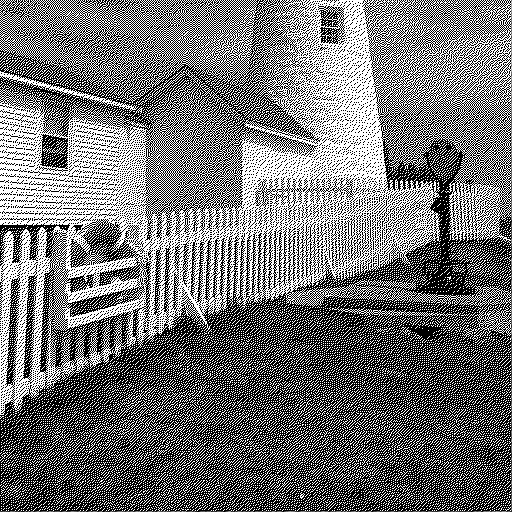
\includegraphics[scale = 0.325]{../Images/Lighthouse/DitheredLighthouse.png}
    \caption{Applicazione dell'algoritmo di Floyd-Steinberg a \emph{Figura \ref{fig:5.1}}}.
    \label{fig:5.2}
\end{wrapfigure}
versione in MATLAB. Si consideri di applicare l'algoritmo all'immagine quantizzata mostrata in \emph{Figura \ref{fig:5.1}},
ciò che si ottiene è mostrato in \emph{Figura \ref{fig:5.2}}.
\begin{center}
    \begin{lstlisting}[language = MATLAB]
        function img = FloydSteinberg(img)
        img = double(img);
        [h,w] = size(img);
        for j=1 : h-1
            for i=1 : w-1
                bin = 255*(img(j,i)>127);
                err = img(j,i)-bin;
                img(j,i) = bin;
                if i<w && j<h
                    img(j,i+1) = 0.375*err+img(j,i+1);
                    img(j+1,i) = 0.375*err+img(j+1,i);
                    img(j+1,i+1) = 0.250*err+img(j+1,i+1);
                elseif i<w
                    img(j,i+1) = img(i,i+1)+err;
                elseif j<h
                    img(j+1,i) = img(j+1,i)+err;
                end
            end
        end
        img = uint8(img);
    \end{lstlisting}
\end{center}
\clearpage

Sebbene ad una prima visione \emph{Figura \ref{fig:5.2} } possa sembrare esattamente \emph{Figura \ref{fig:5.1}}, se osservata da vicino, si nota che le due differiscono.

Si considera ora il caso di un immagine a colore, per farlo si considera \emph{Figura \ref{fig:5.3}.a}.
\subfile{../Figure/Figure 5.3 - Quantizzazione di immagine a colori.tex}
Per prima cosa si applica la quantizzazione alla stessa, risultando nell'immagine di \emph{Figura \ref{fig:5.3}.b}.
Come precedentemente detto la quantizzazione, specie nel caso di immagini a colore, presenta
\begin{wrapfigure}{r}{0.425\textwidth}
    \centering
    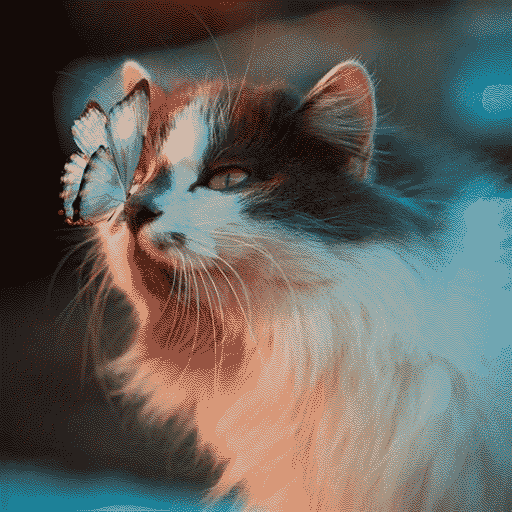
\includegraphics[scale = 0.325]{../Images/Cat/DitheredCat.png}
    \caption{Dithering applicato a \emph{Figura \ref{fig:5.3}.b}.}
    \label{fig:5.4}
\end{wrapfigure}
pattern che risultano sgradevoli, come evidente da \emph{Figura \ref{fig:5.3}.b}.
Applicando adesso il dithering a \emph{Figura \ref{fig:5.3}}, quello che si ottiene è mostrato in \emph{Figura \ref{fig:5.4}}.
Per quel che riguarda il codice MATLAB utilizzato per l'applicazione del dithering, questi è di seguito riportato ed analizzato.
\begin{center}
    \begin{lstlisting}[language = MATLAB]
        % Caricamento di Gatto.png
        [dithered, palette] = rgb2ind(Gatto, 16);
        figure; imshow(dithered, palette); 
    \end{lstlisting}
\end{center}
Passando all'analisi del codice: l'istruzione \lstinline[language = MATLAB]{rgb2ind} restituisce un immagine indicizzata e la relativa palette,
inoltre è possibile passare un terzo parametro per indicare se effettuare dithering o meno.
Qual'ora quest'ultimo è tralasciato di default l'immagine risultante presenterà dithering.

\end{document}